\chapter{Applications to Neuromorphic Hardware}
\label{chapt:results}

Nengo and the NEF provide a useful toolkit for programming recurrently coupled networks of spiking neurons to carry out the computations of algorithms formulated as dynamical systems.
The CPU backend is immensely useful for rapidly prototyping ideas, testing hypotheses, and experimenting with small-scale models on the order of a few thousand neurons.
However, for much larger models such as Spaun~\citep{eliasmith2012}, its 2.5~million neurons require about 2.5~hours of compute time per $1$~second of simulation time, that is $\approx \numprint{9000}$ times slower than real-time~\citep{stewart2014large, mundy2016real}.
As a result, one must turn to specialized hardware such as GPUs, FPGAs, or neuromorphic architectures, in order to carry out much larger simulations of spiking neural networks (section~\ref{sec:neuromorphic}).
For example, in our work in collaboration with \citet{knight2016}, we demonstrated that a heteroassociative memory network (see section~\ref{sec:unsupervised}) deployed on SpiNNaker, took a \emph{constant} amount of time per association, while the exact same network took a linear amount of time per association on a CPU.\footnote{%
The number of neurons scaled linearly in the number of associations.}
At its largest instantiation of \numprint{100000} neurons, the SpiNNaker simulation was more than $150$ times faster than a CPU, due to the massive parallelism afforded by the architecture.

However, there are very few instances of functional large-scale models running on neuromorphic hardware, with \citet{mundy2016real} being the only one that we are aware of to utilize on the order of millions of neurons to do something functionally ``useful''.\footnote{%
Recall this is still five orders of magnitude removed from that of the human brain.}
We believe that this surprising lack of scale---in a field that was essentially created to solve a problem in scaling---is primarily due to a lack of NEF-like frameworks for supporting the robust translation of computations specified in some high-level language (e.g.,~coupled differential equations), onto distributed networks of physically coupled devices.
The Nengo backends for Braindrop~\citep{braindrop2019} and Loihi~\citep{nengoloihi} are brand new---as are the chips themselves~\citep{neckar2018braindrop, davies2018loihi}---and thus currently fall short of their promise to realize \emph{large-scale} functional SNNs in neuromorphic hardware.
For the case of Braindrop, its shortcoming is by design: the chip is $0.65$\,mm${}^2$ and implements $\numprint{4096}$ neurons.
It is a proof-of-concept prototype for research, that can in principle be tiled to scale to much larger models in the future and tailored to the requirements of some application space.
The end-to-end design and fabrication of custom hardware is an extremely costly and complex process that demands a variety of skill-sets from a large number of people.
For the case of Loihi, due to a combination of a lack of hardware support for factorized weight matrices, and limitations on connectivity and memory, the maximum recurrently-connected pool size is $342$ neurons.\footnote{Determined empirically using the \texttt{nengo-loihi==0.6.0} emulator.}
And with current software work-arounds, the precision stops scaling after about $400$ neurons.
On the other hand, this is the first and only software abstraction to currently make use of Loihi, and it is under active development.
We expect this to get significantly better with time.

Nevertheless, these two architectures---Braindrop and Loihi---represent significant milestones in the evolution of neuromorphic hardware.
The first, Braindrop, consumes energy roughly equivalent to $381$\,fJ per synaptic operation, for typical network configurations, or about $10$--$20$ times more than the human brain (see section~\ref{sec:neuromorphic}).
The second, Loihi, consumes about $24$\,pJ per synaptic operation, or about $50$--$100$ times more than Braindrop, but offers determinism and an unparalleled degree of flexibility given its power consumption.
It remains to scale these systems up in useful ways.

Given this discussion, the goal of this chapter is to demonstrate that the fundamentals are in place.
With the guarantees provided by chapter~\ref{chapt:analysis}, the extensions of chapter~\ref{chapt:nef-extensions}, and the functional capabilities of dynamical systems such as those explored in chapter~\ref{chapt:delays} -- we are confident that in principle these methods can scale to Spaun's 6.6~million neurons~\citep{choo2018} and beyond.
However, since we only currently have room for a few hundred neurons, there is only so much that we can do~\citep{blouw2018a}.
Thus, we now demonstrate the principles of the NEF, and a few of its extensions, applied to two fundamental dynamical systems, on the state-of-the-art architectures: Loihi and Braindrop.

\section{Integrator}
\label{sec:integrator}

\begin{figure}
  \centering
  \begin{subfigure}{.5\textwidth}
    \centering
    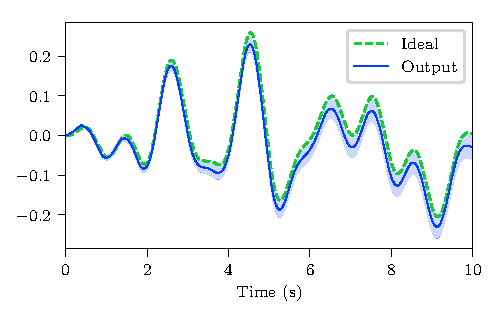
\includegraphics[width=\linewidth]{braindrop-integrator}
    \caption{Braindrop}
    \label{fig:dn-braindrop}
  \end{subfigure}%
  \begin{subfigure}{.5\textwidth}
    \centering
    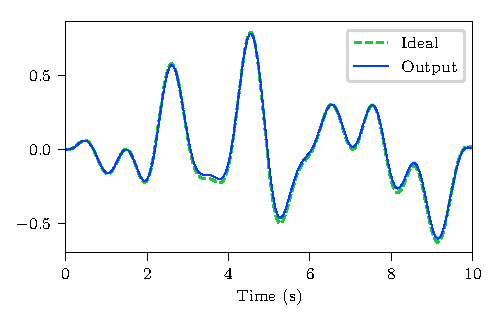
\includegraphics[width=\linewidth]{loihi-integrator}
    \caption{Loihi}
    \label{fig:dn-loihi}
  \end{subfigure}
  \caption[Dynamical integration on Braindrop and Loihi.]{
    An integrator running on state-of-the-art neuromorphic hardware.
    The ideal solution is plotted against the mean's 95\% confidence interval, bootstrapped from $200$ trial simulations.
    (a)~Nengo Braindrop implementation, reproduced from \citet[][Figure~15]{braindrop2019}, using \numprint{1024} neurons. 
    (b)~Nengo Loihi (v0.5.0) implementation, using \numprint{256} neurons.
    Loihi simulations performed by Xuan Choo from Applied Brain Research, Inc.
    See text for details.
  }\label{fig:integrator-neuromorphic}
\end{figure}

The integrator, $\theta \dot{\V{x}}(t) = \V{u}(t)$, is a dynamical system used extensively by Spaun~\citep{eliasmith2012} and many other NEF and SPA models~\citep[][to name a few]{singh2004, trujillo2014a, rasmussen2017} for cognitive tasks involving working memory.
This system persists information about the history of an input signal, starting from $t_0$ and extended indefinitely throughout time, as characterized by the solution to its differential equation,
$$\V{x}(t) = \V{x}(t_0) + \frac{1}{\theta} \int_{t'=t_0}^{t} \V{u}(t')\, dt' \text{.}$$
The parameter $\theta$ is a time-constant that controls how quickly the memory integrates new information.\footnote{
This parameter is useful for dimensional analysis, and when considering the transfer function, $\frac{\V{X}(s)}{\V{U}(s)} = \left( \theta s \right)^{-1}$.}
For example, beginning from an initial state of $\V{x}(t_0) = \V{0}$, if we hold the input constant at $\V{u}(t) = \V{v}$ for $\theta$ seconds ($t_0 < t \le t_0 + \theta$), and then clamp the input to $\V{u}(t) = \V{0}$ thereafter ($t > t_0 + \theta$), then $\V{x}(t) = \V{v}$ will ``store'' the vector $\V{v}$ indefinitely.
More generally, any finite set of nonlinear differential equations can be described as the integration of an input vector that is some nonlinear function of the state-vector---augmented to also include $\V{u}(t)$---as in $\theta \dot{\V{x}}(t) = \V{f}\left({\V{x}(t)}\right)$.
The nonlinearity $\V{f}(\cdot)$ may then be supported by a pool of neurons encoding the state-vector, as explained in section~\ref{sec:nef}.
Thus, the integrator is a basic component that can be used to implement sophisticated nonlinear dynamical transformations, such as those involved in adaptive motor control~\citep{dewolf2016}.
We therefore use the integrator, implemented by a pool of spiking neurons using the methods of the NEF, as a benchmark for evaluating the ability of neuromorphic hardware to implement generic dynamical systems.

In Figure~\ref{fig:integrator-neuromorphic}, we instantiate a one-dimensional integrator ($\theta = 1$\,s) on both Braindrop (1024 neurons) and Loihi (256 neurons).
%\footnote{
%We use four times fewer neurons on Loihi versus Braindrop, as increasing the pool size leads to a bug in the \texttt{nengo-loihi}~v0.4.0 software.}
In both cases, the input signal is a white-noise test signal, band-limited to $1$\,Hz.
Both the ideal and the spiking activity are filtered with a lowpass ($\tau = 200$\,ms).
We report the mean output's 95\% confidence intervals, bootstrapped from $200$ trials.

On Braindrop (see Figure~\ref{fig:integrator-neuromorphic}(a), reproduced from \citet[][Figure~15]{braindrop2019}), we compensate for the distribution of synaptic time-constants, arising from transistor mismatch in the analog circuitry, using the methods of \citet{voelker2017iscas} and section~\ref{sec:mismatch}.
We do this by first measuring the time-constants, and then targetting them individually with the specific transform given by our extension.
The chip is configured to maximize the synaptic time-constants; the empirically measured mean is $179.3$\,ms, with a standard deviation of $53.8$\,ms.

On Loihi (see Figure~\ref{fig:integrator-neuromorphic}(b)), we set $\tau = 200$\,ms, and use the methods of section~\ref{sec:linear-extensions} to discretize the integrator according to the simulation time-step ($\dt{} = 1$\,ms).
We also use non-leaky neurons, as this provides the best accuracy (see section~\ref{sec:poisson-spiking}).
Lastly we move the input synapse onto the spike-generator from host to chip, and uniformly initialize the states of the spike-generators to satisfy the uniform ISIP criteria (Theorem~\ref{thm:correctness}).

In both cases, the 95\% confidence intervals include the ideal across nearly the entire $10$\,s simulation.
This implies that the sum of any error, whether related to spiking, representation, or otherwise, has a mean value of approximately zero.
We remark that Loihi gives much more consistent trial-to-trial results, due to the all-digital nature of the chip, determinism, and lack of temperature-induced variability.
Advanced methods that can be used to provide temperature-invariant decodes in Braindrop have been recently developed by \citet{reidpint2019}, although they require external measurements of the device's temperature, and thus were not employed in this experiment.

\section{Delay Network}
\label{sec:neuromorphic-dn}

\begin{figure}
  \centering
  \begin{subfigure}{.5\textwidth}
    \centering
    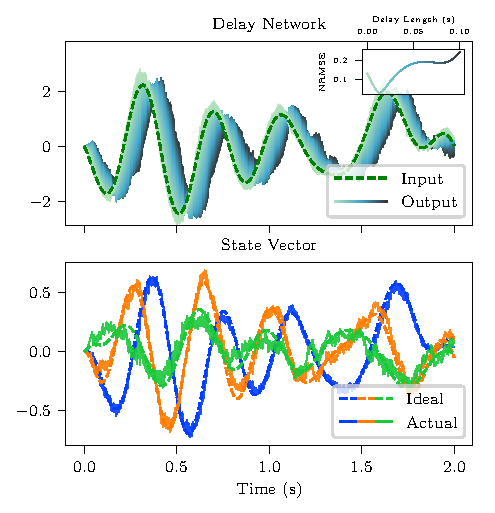
\includegraphics[width=\linewidth]{dn-braindrop}
    \caption{Braindrop}
    \label{fig:dn-braindrop}
  \end{subfigure}%
  \begin{subfigure}{.5\textwidth}
    \centering
    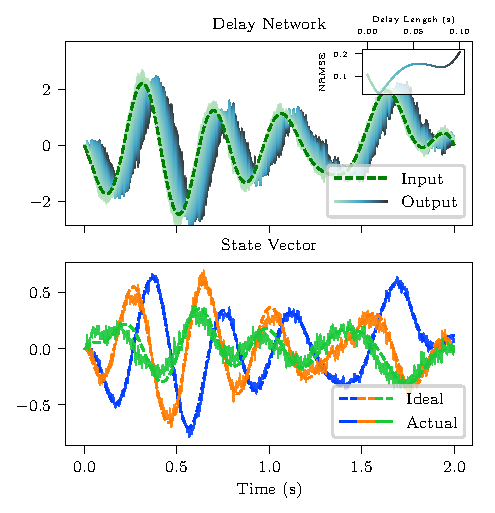
\includegraphics[width=\linewidth]{dn-loihi}
    \caption{Loihi}
    \label{fig:dn-loihi}
  \end{subfigure}
  \begin{subfigure}{\textwidth}
    \centering
    \vspace{2em}
    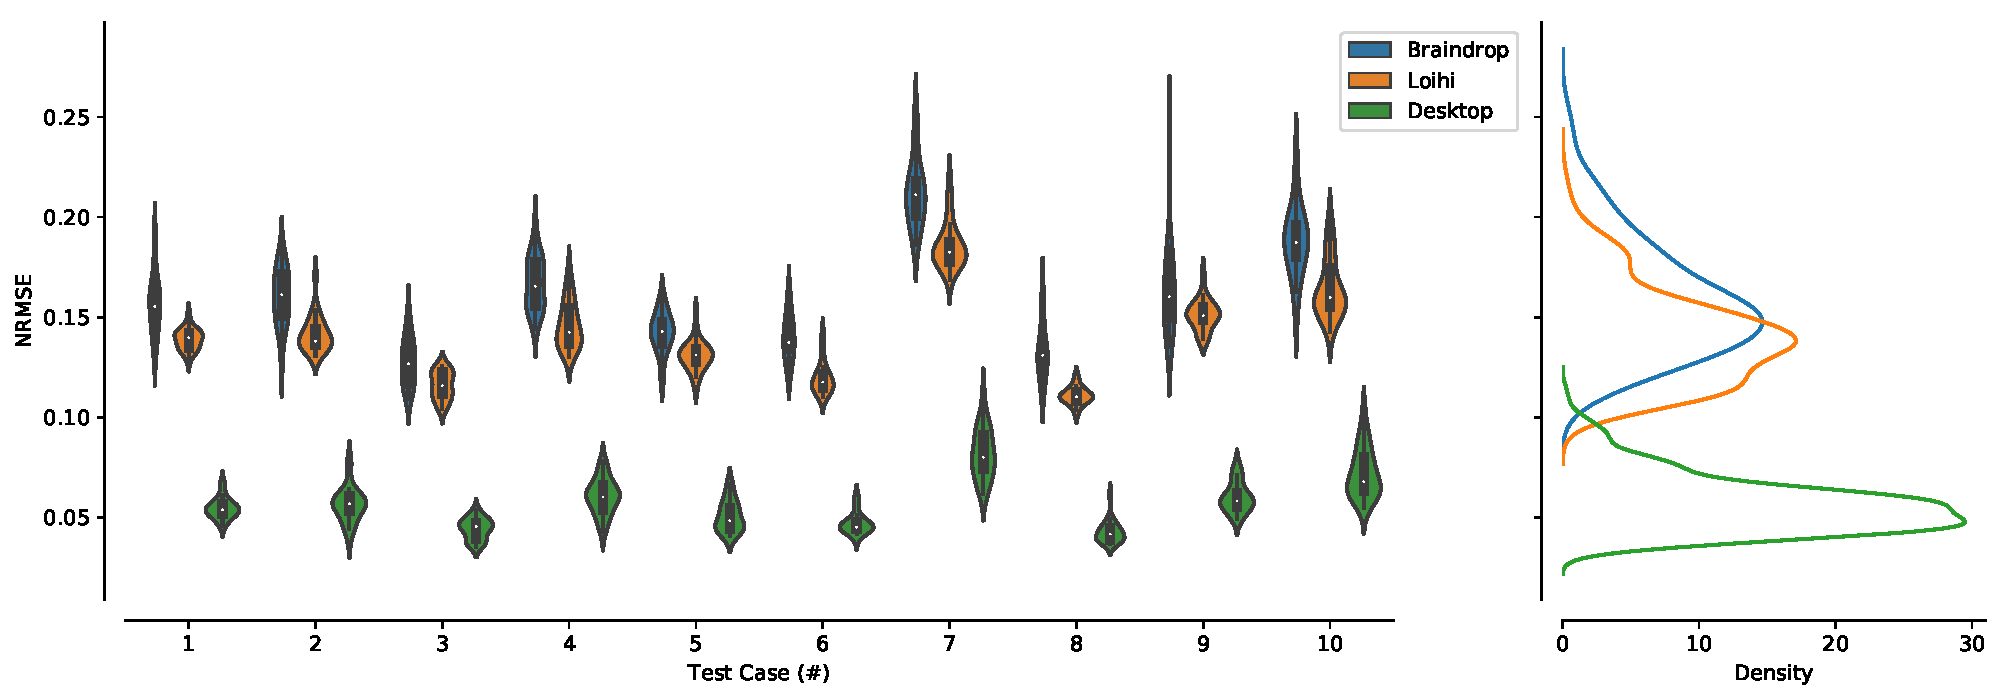
\includegraphics[width=\linewidth]{dn-trials}
    \caption{Overall Error}
    \label{fig:dn-trials}
  \end{subfigure}
  \caption[Dynamical memory on Braindrop and Loihi.]{ \label{fig:dn-neuromorphic}
    Delay Network~(DN; $q=3$, $\theta=100$\,ms; chapter~\ref{chapt:delays}) running on state-of-the-art neuromorphic hardware.
    (a)~Nengo Braindrop implementation, reproduced from \citet[][Figure~16]{braindrop2019}. 
    (b)~Nengo Loihi (v0.5.0) implementation.
    (c)~Overall error~(NRMSE) for Braindrop, Loihi, and a standard desktop CPU.
    The simulations of (a) and (b) correspond to a randomly chosen trial from the first test case from (c).
    Loihi simulations performed by Xuan Choo from Applied Brain Research, Inc.
    See text for details.
  }
\end{figure}

We now instantiate the same Delay Network~(DN) from chapter~\ref{chapt:delays} on state-of-the-art neuromorphic hardware (see Figure~\ref{fig:dn-neuromorphic}).
This system is an entirely different kind of dynamical system that persists not the input's sum, but finite windows of the input's history.
The DN ``buffers'' a sliding window of the input, thus serving as a continuous-time memory, enabling the computation of arbitrary nonlinear transformations across the window.
This can be used as a basic building block for working memory models that must represent not only \emph{what} has occurred, but also \emph{when} it has occurred in relation to everything else.

\TODO{Grab and plot the distribution from the calibration data using the mapped xy coordinates for the 3 ensembles.}

To implement the DN, three pools, each containing $128$ spiking LIF neurons, are recurrently coupled to each other (and to themselves), and trained to optimally buffer a white-noise test signal---band-limited to $3$\,Hz---across a $100$\,ms sliding time-window.
Output spikes are filtered using a lowpass synapse with $\tau = 20$\,ms, and weighted to decode both the state-vector and the window of history using equation~\ref{eq:delay-readouts}.

In this experiment we use identical Nengo model code for both neuromorphic backends.
On Braindrop~(see Figure~\ref{fig:dn-neuromorphic}(a), reproduced from \citet[][Figure~16]{braindrop2019}),
the chip is configured to use the default distribution of synaptic time-constants (mean $\tau \approx 18$\,ms).
For Loihi~(see Figure~\ref{fig:dn-neuromorphic}(b)), the recurrent time-constant is set to $\tau=10$\,ms.
We also compare this to the reference Nengo simulator ($\tau=10$\,ms) running the exact same model on a conventional desktop CPU, to obtain a baseline level of performance.
The overall error, reported as bootstrapped 95\% confidence intervals across $10$ test cases with $25$~trials each, is:
[0.156,~0.163] for Braindrop,
[0.146,~0.153] for Loihi,
compared to [0.145, 0.151] for the Nengo Loihi emulator (not shown), and
[0.055,~0.059] for the CPU (see Figure~\ref{fig:dn-neuromorphic}(c)).

\TODO{ mention in conclusions:
This is remarkable given that spiking reservoirs and FORCE networks cannot achieve these levels of accuracy for the same number of neurons, on a CPU, with additional memory, slower processing, and longer training times (see sections~\ref{sec:delay-rc} and~\ref{sec:force-comparison}).}
